%% ---------------------------------------------------------------------------------------------------------------------

\chapter{Background}\label{ch:background}


%% ---------------------------------------------------------------------------------------------------------------------

\section{Go Unsafe API}\label{sec:background:unsafe-api}

The memory safety measures described in the previous section prevent many of the bugs typical to systems programming
languages.
However, they also take away some flexibility from the developer.
There are legitimate use cases where direct access to the raw memory is required, for example when implementing a
device driver, a network protocol, or an application with tight constrains on resources which needs to convert between
different types without allocating additional memory.
Many memory-safe programming languages like Go, and also Rust, Nim, or even Java offer ways to circumvent the safety
measures provided by the language for those purposes.
In the case of Go, there is the \unsafe{} package~\footnote{\url{https://golang.org/pkg/unsafe}}, an \acrshort{API} that
allows developers to use raw pointers with all their benefits and dangers.

\begin{lstlisting}[language=Golang, label=lst:unsafe-api, caption=\textit{Unsafe} package API]
package unsafe

type Pointer

func Alignof(x ArbitraryType) uintptr
func Offsetof(x ArbitraryType) uintptr
func Sizeof(x ArbitraryType) uintptr
\end{lstlisting}

Listing~\ref{lst:unsafe-api} shows the \acrshort{API} of this package.
It contains \checkNum{three} functions \textit{Sizeof}, \textit{Alignof}, and \textit{Offsetof} (Lines~5--7),
as well as the type \textit{Pointer} (Line 3).
The \textit{unsafe.Pointer} is the most important package member.
It is a pointer type in the sense that the garbage collector follows it to determine live references, but apart from
that the normal restrictions for memory safety do not apply.
In particular, unsafe pointers can be converted to and from any other pointer type, allowing arbitrary casts between
any type.
Furthermore, they can be converted to and from \textit{uintptr} values, which is an integer type with sufficient size
to store pointers on the specific target architecture of the program.
Since \textit{uintptr} values behave like normal integer variables, they can be used in arithmetic expressions.
Therefore, unsafe pointers can also be used to achieve pointer arithmetic.
With \textit{unsafe.Pointer}, developers can achieve the same flexibility as with raw \textit{void*} pointers in C.

Listing~\ref{lst:unsafe-examples} shows examples of both \textit{unsafe.Pointer} features.
The \textit{floatToBits} function (Line~3) illustrates how the variable \textit{x} of type \textit{float32} is first
cast to an unsafe pointer and then to a value of type \textit{int} (Line~4).
Since the unsafe conversion rules only allow arbitrary casts between any pointer type, \textit{x} is first converted
into a pointer value and the resulting \textit{int} pointer is dereferenced before returning the final value.
This conversion yields the raw bits of the floating point value stored using the IEEE 751 format.
It would be impossible using the normal Go conversion rules because \textit{float32} and \textit{int} are incompatible
types.
The \textit{secondByte} function (Line~7) shows how pointer arithmetic is used to manually iterate over an array type.
The function expects an array of size five bytes and returns the second byte.
Instead of direct indexing, it achieves this by obtaining the address of the array as a \textit{uintptr} value, adding
1 and then casting the resulting address to a \textit{byte} value, again taking care of dereferencing the resulting
pointer type (Line~8).

\begin{lstlisting}[language=Golang, label=lst:unsafe-examples, caption=Usage examples of the Go \textit{unsafe} API]
import "unsafe"

func floatToBits(x float32) int {
    return *(*int)(unsafe.Pointer(&x))
}

func secondByte(b [5]byte) byte {
    return *(*byte)(unsafe.Pointer(uintptr(unsafe.Pointer(&b)) + 1))
}
\end{lstlisting}

It is important to note that while \textit{unsafe.Pointer} is a pointer type, \textit{uintptr} is not.
This means that addresses that are stored in variables of type \textit{uintptr} are not treated as references by the
garbage collector, and thus values referenced by it can get freed although there are still live references.
Possible consequences of this are described in Chapter~\ref{ch:unsafe-security-problems}.
Other dangers include that accessing raw bytes of data structures exposes low-level implementation details such as
the alignment of structure fields to word-bound addresses, which can change with future versions of the Go compiler or
runtime and thus break programs when they are not carefully updated later on.
In general, using the \unsafe{} package must be done with caution and should be avoided whenever possible.

The other functions of the \unsafe{} packages are evaluated at compile time and can be used to gain knowledge about
the size, alignment, or offset of a field in a structure type relative to the start of the structure.
These can be necessary when dealing with the direct byte representation of structure types such as when implementing
network protocols or device drivers.
In this thesis the term \unsafe{} usage refers to all members of the \unsafe{} package as well as the slice and string
header structures that are described in more detail in Chapter~\ref{ch:unsafe-security-problems}.

%% ---------------------------------------------------------------------------------------------------------------------

\section{Slices and Strings in Go}\label{sec:background:slices}

Slices in Go are an array data type consisting of an underlying memory area and information about length and capacity.
The length indicates how many elements are currently contained in the slice, and the capacity denotes the allocated
space in memory.
When a subset of the slice is taken by specifying start and end indices, then a new slice is created that uses the same
underlying data array as the original one, and might have a capacity longer than its length if there are further
elements in the original slice after the end of the newly-taken subslice.
It is possible to increase the size of the new slice up to its capacity, but the size can never be larger than the
capacity.
When new elements are added to a slice using the \textit{append} function, then a new slice is created too which has a
higher length than the previous.
The runtime reuses the underlying data array of the original slice as well if its capacity is big enough, or allocates
a new array for the new slice if it is not.
Strings in Go are read-only \textit{[]byte} slices.
Usually they are encoded in UTF-8, but this is not required.
The length of a string is always the number of bytes needed to store its encoded form, which is often not the same as
the number of characters in the string.
It is important that strings are immutable because string literals are placed in a constant data section of the binary
when the code is compiled, meaning they are usually located within a read-only memory page and mutating them would cause
the program to receive a segmentation fault signal and crash.

\begin{lstlisting}[language=Golang, label=lst:reflect-header-types, caption=Reflect slice and string header types and API]
package reflect

type SliceHeader struct {
    Data uintptr
    Len int
    Cap int
}

type StringHeader struct {
    Data uintptr
    Len int
}
\end{lstlisting}

It is possible to access the internal structure of slices and strings by casting them to their header representation
using the \unsafe{} \acrshort{API}.
Listing~\ref{lst:reflect-header-types} shows the \acrshort{API} of these header types.
As the name suggests, slices correspond to the \textit{SliceHeader} type (Line~3), while strings are associated with the
\textit{StringHeader} type (Line~9).
The \textit{Len} fields (Lines~5 and ~11) denote the current length of the slice or string, and finally the
\textit{SliceHeader} type has an additional \textit{Cap} field (Line~6).
It stores the allocated capacity of the slice, which is the available size it can grow to until its data array must be
reallocated when new elements are added.
Notice that the reference to the underlying data array has the type \textit{uintptr} in both types (Lines~4 and~10),
therefore it is not inherently treated as a pointer type by the garbage collector (\acrshort{GC}).
Instead, there is a special case in the Go runtime that recognizes slices and strings and follows the address stored in
the \textit{Data} field to prevent it from getting collected.
To prevent these dangers, many programming languages provide features to achieve a higher level of memory safety.
There can be compile-time or static measures, runtime or dynamic measures, or a combination of both.
The Go programming language uses automatic memory management, which means that developers do not need to manually
allocate and free memory for data structures, instead a value is simply declared and the compiler adds the code to
properly allocate the appropriate space in memory.
Furthermore, the Go type system prevents invalid conversions between incompatible types, such as data structures with
different size.
Buffers can be expressed either as arrays with fixed length, or slices.
In the case of arrays, the type system encodes the length of the buffer as a type information, for example instances
of \textit{[10]byte} and \textit{[20]byte} have fundamentally different types and can not be converted into each other
or passed to a function that expects a buffer of different length.
In contrast, in C it would be common to pass around a pointer to the beginning of the buffer, which would not carry
information about the length.
In the case of slices, they are represented by a header structure containing information about the allocated size as
well as a pointer to the underlying data, which will be described in slightly more detail in
Chapter~\ref{ch:unsafe-security-problems}.
The Go runtime takes care that there can not be any accesses outside the slice bounds.


%% ---------------------------------------------------------------------------------------------------------------------

\section{Memory Management}\label{sec:background:memory}


%% ---------------------------------------------------------------------------------------------------------------------

\subsection{Stack and Heap}\label{subsec:background:memory:stack-heap}

The working memory of a computer, more specifically the Random Access Memory (\acrshort{RAM}) is used to hold both
application data and program instructions.
It is essentially a single string of bytes that each have an increasing address.
To organize this memory effectively, it is divided into memory pages that can get mapped into virtual memory sections.
These sections and pages are managed by the operating system (\acrshort{OS}).
Virtual memory allows each process to address its data regardless of its actual position in the physical memory.
When a process is loaded by the \acrshort{OS}, its execution will always start at the same virtual address which is
stored in the executable file.
The \acrshort{OS} will then take care of translating the virtual address into an actual absolute memory address.
The virtual memory of a process is further divided into different functional areas, most importantly the text sections,
the heap, and the stack.

The text sections contain the machine-readable program instructions.
The heap is a data section that stores data with a lifetime greater than a single function, for example global
variables.
Memory can be allocated there using dedicated runtime functions like \textit{malloc} in C and must be freed after it is
not needed anymore to avoid running out of heap memory.
Finally, the stack is also a data section, but in contrast to the heap it is used for local variables of functions, as
well as their arguments and possibly return values.
The stack pointer register (\textit{rsp} in the \textit{amd64} architecture) in the processor stores the current top
of the stack, which is the address of the last value that was added to the stack.
If a new value is pushed, then the stack pointer is decremented and the data can be written to its new address.
It is possible to decrement the stack pointer by any number of bytes to make room for several variables at once, and
then those variables can be accessed by adding a fixed offset to the stack pointer.
Because the active, allocated stack memory is always at addresses equal or higher than the stack pointer, and adding
new data means the value of the stack pointer is reduced, the stack grows from the top of the memory to the bottom.
Figure~\ref{fig:stack} shows a visualization of the concept of pushing data to the stack.

\begin{figure}[htp!]
    %\vspace{2mm}
    \centering
    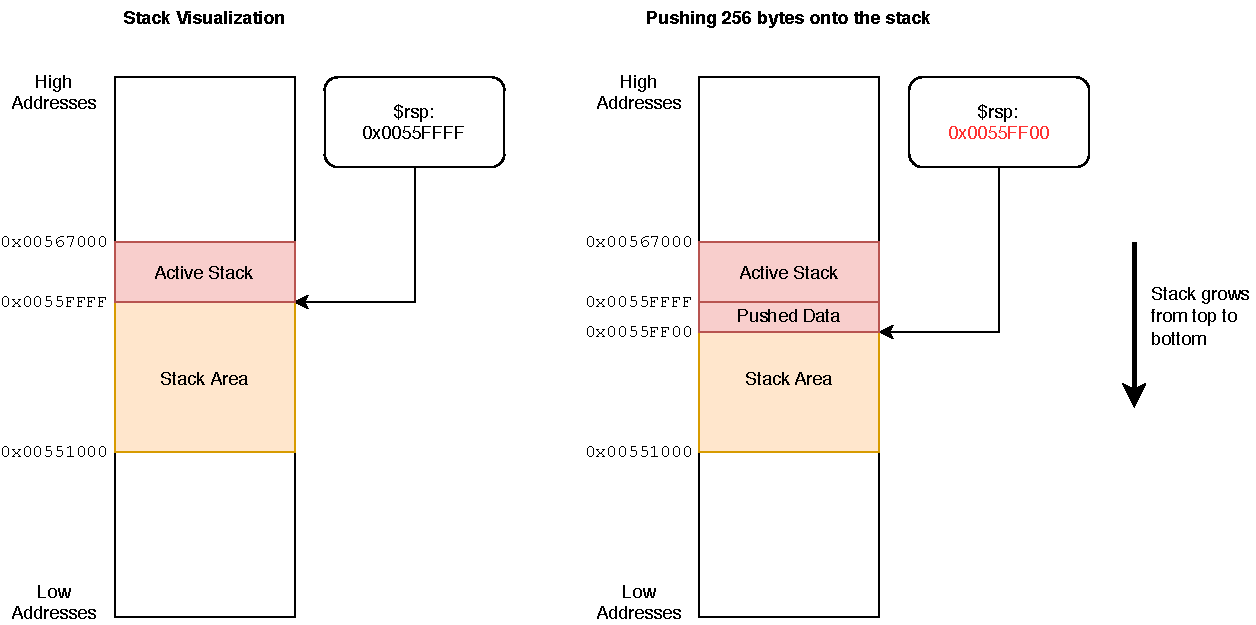
\includegraphics[width=\textwidth]{assets/figures/stack.pdf}
    \caption{Pushing to the Stack}
    \label{fig:stack}
    %\vspace{-10pt}
\end{figure}


The stack itself is organized in frames.
When a function is called, a new stack frame is created for this function.
The caller function starts setting up the parameters of the callee.
How this is done depends on the specific architecture that the program is run on, as well as the calling convention,
which together form the Application Binary Interface (\acrshort{ABI}).
Figure~\ref{fig:stack-frame-layout} shows an example stack frame for a C function call.
The source code for the function is included in the figure.
The stack frame is using the \textit{amd64} 64-bit Linux calling convention.

The first six parameters of the \textit{example} function are passed in registers, but the last two are pushed on the
stack in reverse order.
Next, the address of the next instruction of the caller function, that is the address that the callee should return
to after it has finished, is saved on the stack.
This allows to chain function calls, including recursion, because returning simply removes the stack frame and jumps
to the saved return address of that frame.
The return address marks the end of the caller stack frame, after that begins the callee stack frame for the new
function.
It starts by saving the current state of the processor registers so that the function can use them for calculations and
later restore their values to the original ones expected by the caller function.
After that, local variables of the function are allocated on the stack.
In this example, they are placed in the order of definition in the source code, but that is not a requirement.
The compiler will decide how to place the local variables and keep track of their addresses as relative offsets to the
stack pointer register.
When the function returns, the stack pointer will be incremented by the size of the callee stack frame, and then the
return address will be fetched and put into the instruction pointer register.
The return value of the function is passed in a register in this example.
In a Go program, returning values can also be achieved using the stack, which the compiler does in the case of multiple
return values.

\begin{figure}[htp!]
%\vspace{2mm}
\centering
    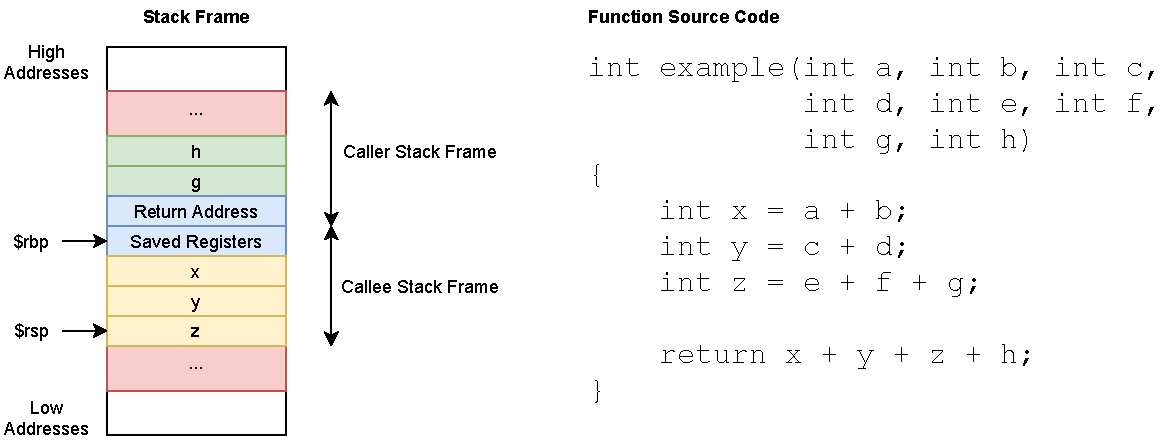
\includegraphics[width=\textwidth]{assets/figures/chapter2/stack-frame-layout.pdf}
    \caption{Stack Frame Layout}
    \label{fig:stack-frame-layout}
    %\vspace{-10pt}
\end{figure}



%% ---------------------------------------------------------------------------------------------------------------------

\subsection{Escape Analysis (EA)}\label{subsec:background:memory:ea}

\acrshort{EA} is used to decide whether a variable can be placed on a function's stack or needs to be allocated on the
heap.
The stack is preferred because there is no explicit deallocation step needed to free the stack memory, instead the stack
frame is removed completely when the function returns as described in Section~\ref{sec:background:memory-safety-layout}.
In \acrshort{EA}, a value is said to escape if references to it can live longer than the current function's lifetime.
If it does escape, then it needs to be allocated on the heap so that when the function has terminated, references that
still exist can continue to access the memory even though the function stack has vanished.
Otherwise, it can be placed on the stack.
The \acrshort{EA} analysis employed by the Go compiler works by checking for each variable that is declared in a
function whether a reference to it is stored in another value or passed to another function.
If there is a reference stored in another object, this object has to be checked too, and if it escapes then so does the
original variable.
The same is true for functions: if the variable gets passed to another function then the \acrshort{EA} algorithm
transitively looks into that function and determines if the value escapes there.
If it does, then it must also be treated as an escaped value in the original function.
Finally, if the function returns a reference to the variable then it obviously escapes as well.


%% ---------------------------------------------------------------------------------------------------------------------

\subsection{Garbage Collection (GC)}\label{subsec:background:memory:gc}

The Go runtime uses a garbage collector (\acrshort{GC}) that analyzes which values can still be referenced by active
pointer values, and automatically frees all unreachable values.
This technique prevents \textit{use-after-free} vulnerabilities because there is no explicit deallocation.
Go uses a move-and-sweep GC that runs concurrently with all other threads of a program to free unused heap
memory~\cite{sibiryov2017}.
It is triggered by one of two conditions, either when the heap usage has increased to a specific size (usually when the
usage has doubles since the last \acrshort{GC} run), or after a fixed time has passed without any \acrshort{GC} runs.
The \acrshort{GC} takes all variables that are present in the scope of the program and marks them as live.
Then, it recursively follows all pointer types within live variables and marks their target values as live, too.
After this marking phase has completed, the sweep phase frees all memory that is not marked as live.
Finally, the markings are reset and a new \acrshort{GC} run can be triggered.

Figure~\ref{fig:gc-visualization} shows a visualization of the marking phase in a \acrshort{GC} run.
The variables in scope can be either on the stack, which is not managed by the \acrshort{GC}, or on the heap, in which
case they are marked as being live as well.
The arrows indicate references from pointer types to their targets, and the blue values on the heap are the ones marked
as live.
The white heap values will be freed in the sweep phase of the \acrshort{GC}.

\begin{figure}[htp!]
    %\vspace{2mm}
    \centering
    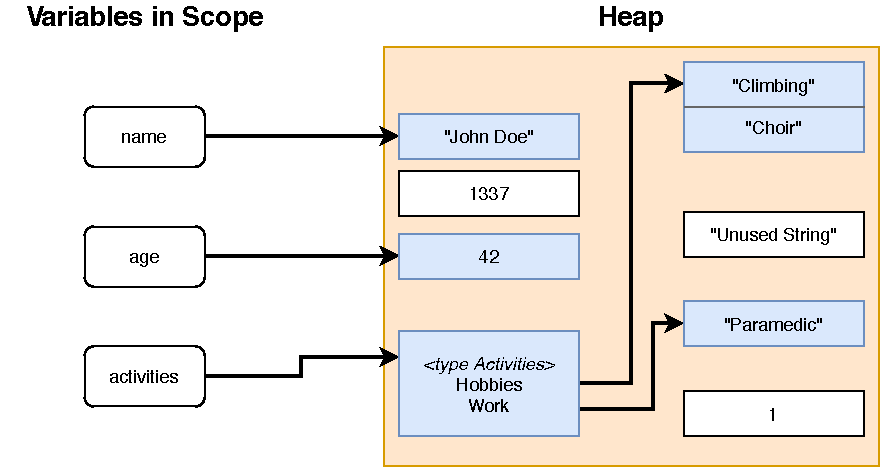
\includegraphics[width=0.6\textwidth]{assets/figures/chapter3/gc-visualization.pdf}
    \caption{Garbage Collector Visualization}
    \label{fig:gc-visualization}
    %\vspace{-10pt}
\end{figure}



%% ---------------------------------------------------------------------------------------------------------------------

\section{Exploit Techniques and Mitigations}\label{sec:background:exploit-techniques}

A frequent security vulnerability in programs that use traditional systems languages like C are buffer overflows.
They happen when an array variable, for example a string, is too short for the data that is written to it, causing the
data to overflow into and overwrite adjacent memory.
Overflows can happen anywhere in the memory, however a common source of security problems are stack-based buffer
overflows.
When a buffer variable is placed on the stack and too much data gets written to it, the data will be written to higher
memory addresses, which means after overwriting the other local variables and saved registers they can cause the saved
return address to get changed.
When an attacker can control the data that is placed there, they can change the program flow by carefully choosing the
address that ends up being jumped to after the current function returns.

A common problem with data placed on the heap is that if it gets freed but then the program continues to try and use the
data, it is possible that the memory at that address has already been reused and new data is accessed, potentially
reading or writing data from another thread.
However, the same can happen with data on the stack if there are references to the data that remain after the stack
frame has been destroyed, as dereferencing that address can then access memory that belongs to a different frame and
thus potentially change arbitrary data including the saved return address.
This kind of problem is called \textit{use-after-free}.


%% ---------------------------------------------------------------------------------------------------------------------

\subsection{Buffer Overflow}\label{subsec:background:exploit-techniques:buffer-overflow}

Buffer overflows and \textit{use-after-free} vulnerabilities are a very common root cause for security problems in
traditional systems programming languages, as those usually offer direct access to the memory in terms of raw pointers
and manual allocations~\cite{larochelle2001}.
The most basic approach to inject arbitrary code is to place machine instructions into the exploit input data, which
will then be written to the stack.
They can be before or after the address that gets overwritten at the position of the saved return instruction pointer,
but usually it is placed after because there is more space available.
The instruction pointer is then set to the start address of the machine instructions payload.
Since stack addresses can be slightly unpredictable in practice, for example because environment variables with
different lengths might be located on the stack, a \textit{NOP-slide} can be used to make the exploit more robust.
\textit{NOP}, or \textit{no-op}, is a machine instruction that does nothing at all, the processor simply continues with
the following instruction.
A \textit{NOP-slide} then is a series of such instructions.
Using this, it is sufficient to overwrite the return instruction pointer with an address somewhere within the
\textit{NOP} instructions to make the processor go through all remaining of them until it reaches the exploit code,
similar to sliding down a slope.
Thus, the address does not have to match the exact start of the payload code anymore, instead it can have a tolerance.
Figure~\ref{fig:stack-smashing-payload} shows a visualization of an example input data used to spawn a shell that an
attacker can then use to execute arbitrary code.

\begin{figure}[htp!]
    %\vspace{2mm}
    \centering
    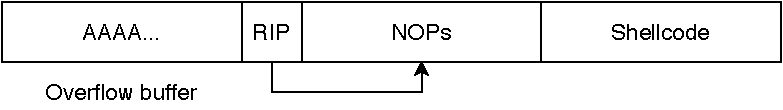
\includegraphics[width=0.8\textwidth]{assets/figures/chapter2/stack-smashing-payload.pdf}
    \caption{Stack smashing payload to inject exploit code}
    \label{fig:stack-smashing-payload}
    %\vspace{-10pt}
\end{figure}



%% ---------------------------------------------------------------------------------------------------------------------

\subsection{Data Execution Prevention (DEP)}\label{subsec:background:exploit-techniques:dep}

However, such a type of exploit does not work an modern operating systems because they employ mitigation techniques
against this.
Executing machine instructions that are placed in memory that is part of the stack is prevented because the memory pages
containing the stack are marked as non-executable.
This technique is called Data Execution Prevention (\acrshort{DEP}).
It takes care of having sections in memory be either executable or writable, but not both.
That way, attackers can not easily write code into the memory and then jump into this code.


%% ---------------------------------------------------------------------------------------------------------------------

\subsection{Address Space Layout Randomization (ASLR)}\label{subsec:background:exploit-techniques:aslr}

To work around \acrshort{DEP}, attackers can reuse existing functions in the binary, because as part of the text section
these are located on executable (but not writable) memory pages.
There is Address Space Layout Randomization (\acrshort{ASLR}), which loads dynamically-linked libraries into random
memory positions to avoid having predictable function addresses usable by attackers for code that is part of standard
libraries, like the C library \textit{glibc}.
However, \acrshort{ASLR} does not apply to statically-linked code, which the Go compiler mostly creates.


%% ---------------------------------------------------------------------------------------------------------------------

\subsection{Return Oriented Programming (ROP)}\label{subsec:background:exploit-techniques:rop}

Return-oriented programming (\acrshort{ROP}) is a specific technique for reusing code that suggests jumping to very
small so-called gadgets, which are sequences of two or few more machine instructions that do not modify the stack
pointer register and end with a return instruction \jl{add citation}.
With these properties, gadgets can be chained because after the execution of a fragment the return instruction fetches
the next address to jump to from the stack, which the attacker can control.
Depending on the available \acrshort{ROP} gadgets, the attacker can therefore concatenate them and thus write a program
with a limited set of assembler instructions available.
The Go standard library is very large and thus provides many available gadgets.
This makes exploiting a buffer overflow, once it exists in a Go program, even easier compared to a C program where an
attacker would have to work around \acrshort{ASLR}, for example.


%% ---------------------------------------------------------------------------------------------------------------------

\section{Dependency Management in Go}\label{sec:background:dependencies}

To break code into logical units that can be maintained separately and allow reusing them, Go offers a dependency
management system.
The smallest possible unit is a Go package.
A package can contain one or more source code files which must all be in the same directory.
It has a name which should match the name of the directory containing the source files.
There can not be more than one package in the same folder.
Identifiers such as function and variable names must be unique in the scope of the same package and can be accessed
directly.
Therefore, developers can split their code into individual code files without restrictions to organize a single package.
When accessing code in a different package, the package name must be used as prefix in front of the identifier name.
Furthermore, the package must be imported using an \textit{import} statement at the beginning of the file.
Package imports are valid only within a file, not a whole package, and thus must be repeated in all files that access
the external package.
It is only possible to access exported fields from another package, which is indicated by starting the identifier with
a capital letter.
When importing the package, it is necessary to specify the complete path to the package, the name is not sufficient on
its own.
The import path is made up of the directory tree leading to the package directory, separated by forward slashes.
For example, a valid import path would be \textit{my-application/storage/database}.


%% ---------------------------------------------------------------------------------------------------------------------

\subsection{GOPATH and GOROOT}\label{subsec:background:dependencies:gopath}

To allow sharing code with other developers and implementing reusable libraries, it is possible to download external
packages using the \textit{go get} command, which can fetch packages using \acrshort{HTTP}, Git, or other means.
The import path usually begins with a \acrshort{DNS} host such as \textit{github.com} which hosts the package code.
The host part is then called \textit{registry}.
However, a drawback is that this technique does not allow to specify a version of the imported package, which makes it
very hard to publish stable libraries.

\todo{Explain GOPATH and GOROOT}


%% ---------------------------------------------------------------------------------------------------------------------

\subsection{Go Module System}\label{subsec:background:dependencies:modules}

Starting with the release of Go \checkNum{1.11}, the development of the module system has fixed this by introducing a
new unit of code organization.
Modules contain one or more packages, and have a name and import path similar to packages, which can in fact be the name
of a root package in the module.
Furthermore, modules are required to be available as a revision control repository like Git and are versioned.
A project can define dependencies to specific versions of other modules, which resolve to the packages imported in the
code.
Thus, it is possible to require a specific version of an external package.
Dependencies can be transitive, because imported modules can have dependencies to other modules themselves,
forming a dependency tree.
Figure~\ref{fig:dependency-model} shows an example of the relations between the different units of code organization
used in Go.
The \textit{github.com/example/example} module is the main application module and its current version is
\textit{v2.0.0}.
It contains three separate packages \textit{A}, \textit{B}, and \textit{C}, all of which are composed of individual Go
source files.
The module depends upon two other modules \textit{X} and \textit{Y}, both of which are imported with a specific version.
These again contain one or more packages with source files, and further depend on more modules.
The \textit{Y} module is effectively imported in two different versions, \textit{v1.0.1} and \textit{v5.3.0}, so both
their sources will be compiled and included in the resulting binary.

\begin{figure}[htp!]
    %\vspace{2mm}
    \centering
    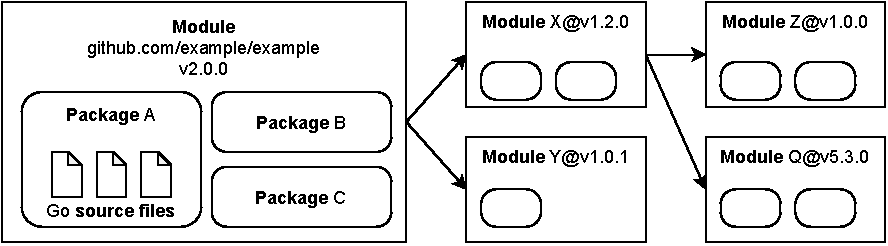
\includegraphics[width=\textwidth]{assets/figures/chapter2/dependency-model.pdf}
    \caption{Dependency management model used by Go}
    \label{fig:dependency-model}
    %\vspace{-10pt}
\end{figure}


Projects lock their dependencies including versions in a file called \textit{Go.mod}.
When the code is built, the Go compiler toolchain will automatically figure out which modules need to be downloaded and
get the code.
There are however still many projects that do not use the module system and \textit{Go.mod} file yet, because it is only
stable since recently with the release of Go \checkNum{1.13} in \checkNum{September 2019}.


%% ---------------------------------------------------------------------------------------------------------------------

\section{Static Code Analysis}\label{sec:background:static-code-analysis}

Static code analysis describes techniques that examine source code for particular properties, such as code metrics or
the presence of specific bugs, without running the program.
In the last point, it is different from dynamic code analysis which executes the code and employs runtime checks.
Using static code analysis, it is possible to automatically test if the source code matches certain expectations.
Based on the level of abstraction that an analysis tool is looking at, it can be classified into lexical, syntactic,
or semantic analysis.
Lexical analysis deals with the source code as text, with the most common purpose being coding style enforcement.
For syntactic analysis, the code is parsed to obtain an abstract syntax tree (\acrshort{AST}), which allows for example
to do type checking and reporting code metrics such as the cyclomatic complexity or McCabe metric~\cite{watson1996} or
the number of \unsafe{} usages, as described in Chapter~\ref{ch:go-geiger}.
Finally, semantic analysis also takes care of the control and data flow, which describe what statements in the code can
be executed in which order and how data is being transferred between variables.
This allows for example to detect unused or dead code, or detect whether a variable is used before it is initialized.
To do this, a control flow graph (\acrshort{CFG}) is used.


%% ---------------------------------------------------------------------------------------------------------------------

\subsection{Abstract Syntax Tree (AST)}\label{subsec:background:static-code-analysis:ast}

Figure~\ref{fig:ast} shows an example of an \acrshort{AST}.
It represents a code fragment of just one statement, which is \textit{x := 3 + 5}.
Source code of programming languages is a formal language that follows a grammar, which is its syntax.
Syntactically valid programs are words in the formal language and can be represented as the tree of grammar rules used
to construct the word.
Such a grammar construction begins with a start symbol, such as \textit{AssignStmt} in this case.
It can have children, which are recursively substituted for concrete values.
In Figure~\ref{fig:ast}, the right hand side of the assignment is an addition, an instance of a binary expression, with
basic integer literals 3 and 5 used for the addition.
The \acrshort{AST} shows the composition of the source code into logical units of growing size, with the leafs being
identifiers, literals, or any other nodes that do not contain further children, such as an empty return statement for
example.
To obtain the \acrshort{AST}, it is possible to use the standard parser bundled with the language's compiler.
An advantage of running static analysis steps on the \acrshort{AST} is that it is independent from any concrete lexical
representation such as white space.
Identifier names can also be easily replaced by different names in the abstract representation, which makes the
\acrshort{AST} perfect for name refactoring operations or recognizing specific types even if they are aliased in the
source code.

\begin{figure}[htp!]
    %\vspace{2mm}
    \centering
    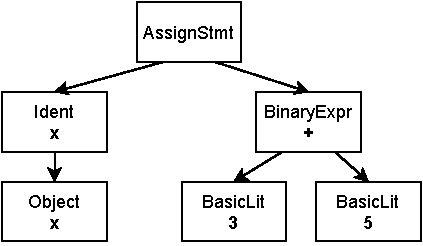
\includegraphics[width=0.5\textwidth]{assets/figures/chapter2/ast.pdf}
    \caption{Abstract syntax tree visualization for source code "x := 3 + 5"}
    \label{fig:ast}
    %\vspace{-10pt}
\end{figure}



%% ---------------------------------------------------------------------------------------------------------------------

\subsection{Control Flow Graph (CFG)}\label{subsec:background:static-code-analysis:cfg}

In contrast, the \acrshort{CFG} is not purely based on syntax anymore, but needs semantic analysis to be constructed.
It is a directed graph showing possible execution paths through the code segments.
It can contain cycles and is not necessarily connected (neither strongly nor weakly).
Nodes in the control flow graph denote logical pieces of the source code in the sense that they form a unit of
execution.
They can be seen as an atomic step of computation.
While \acrshort{CFG} nodes are also nodes in the \acrshort{AST}, there are \acrshort{AST} nodes that are not a
\acrshort{CFG} node.
Edges in the \acrshort{CFG} then represent all possible paths of execution.
An example of a \acrshort{CFG} can be seen in Figure~\ref{fig:cfg}.
It shows a simple loop: \textit{for x < 5 \{ x += 1 \}}.

\begin{figure}[htp!]
    %\vspace{2mm}
    \centering
    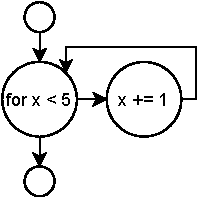
\includegraphics[width=0.25\textwidth]{assets/figures/chapter2/cfg.pdf}
    \caption{Control flow graph for source code "for x < 5 \{ x += 1 \}"}
    \label{fig:cfg}
    %\vspace{-10pt}
\end{figure}


There are two logical steps of execution in this code example.
After any previous code is executed and control flows to the \textit{for} loop, first the loop condition \textit{x < 5}
is checked.
Then, there are two outgoing edges on the node because the condition can be either true or false.
If it is true, then control flows to the assignment node representing the \textit{x += 1} statement.
That node then has an edge back to the loop condition node to check whether the loop should be run again.
Otherwise, the code following behind the loop is executed.
Such a \acrshort{CFG} is an excellent tool to detect dead code, which would be represented by an isolated connectivity
component in the graph.
Furthermore, using node annotations that indicate whether variables are read or assigned, it is possible to detect
control flow anomalies such as read-before-write, which would show that a variable is used before it is initialized.
It is also useful to detect where a variable is assigned for the last time before a particular statement, thus what
value it has at time of execution of that statement.


%% ---------------------------------------------------------------------------------------------------------------------

\subsection{Go Linters \toolVet{} and \toolGosec{}}\label{subsec:background:static-code-analysis:linters}

There are a number of existing static code analysis tools for the Go programming language.
The most official is \toolVet{}\footnote{\url{https://golang.org/cmd/vet}}, which is included as part of the main Go
\acrshort{CLI} and thus is installed by default with the Go compiler.
As described in more detail in Section~\ref{sec:go-safer:implementation} about the implementation of \toolSafer{}, it
is built using a modular system of individual analysis steps.
Examples of these steps include checking if returned values from functions are unused, type checking of the format
specifiers used in the \textit{fmt.Printf} function with respect to the concrete parameters, or detecting unreachable
code.
Another static analysis tool with a focus on security is \toolGosec{}\footnote{\url{https://github.com/securego/gosec}}.
Similar to \toolVet{}, it contains a number of different rules that the source code is checked against, for example if
insecure hash functions are used, template strings contain unescaped data, or returned error values from functions are
actually checked.
Such static analysis tools that detect insecure code or common mistakes are called linters.

